%interface membre
\subsubsection{Analyse}

Le r\^{o}le  du membre consiste à modifier  l`\'{e}tat et la progression d'une t\^{a}che .
 \textbf{ Diagramme de cas d'utilisation "G\'{e}rer une t\^{a}che "}
    \begin{figure}[H]
    \center
    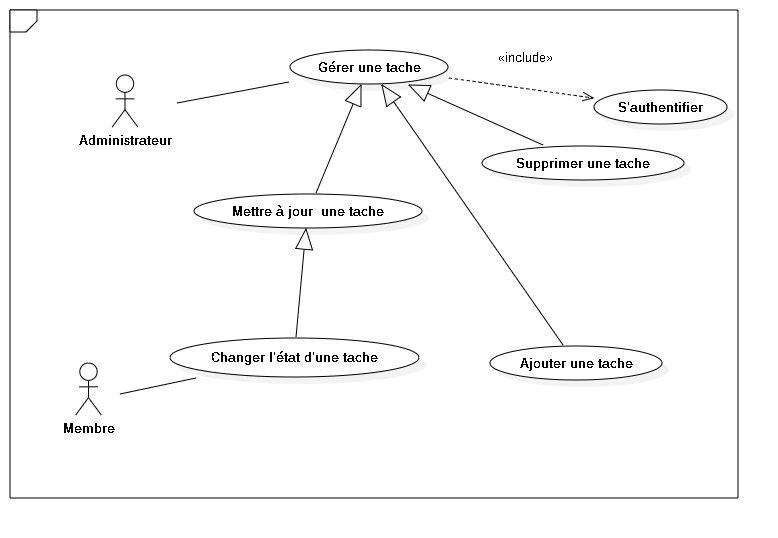
\includegraphics[width=13cm,height=8cm]{./figures/ucT.png}
    \caption{G\'{e}rer une  t\^{a}che.}

    \end{figure}

\subsubsection{Conception}
\textbf{ Le sc\'{e}nario \guillemotleft{} Modification de l`\'{e}tat d'une t\^{a}che\guillemotright{}}

Le diagramme de s\'{e}quence \guillemotleft{} Ajout d'une t\^{a}che \guillemotright{} pr\'{e}sente le s\'{e}quencement
des interactions entre Administrateur, Application et Base de donn\'{e}es (BD).


\begin{figure}[H]
\center
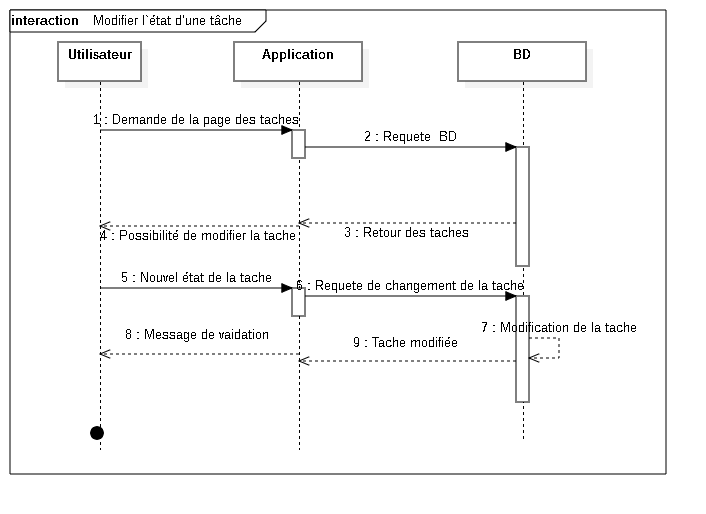
\includegraphics[width=14cm,height=10cm]{./figures/seq/D.png}
\caption{ Modification de l`\'{e}tat d'une t\^{a}che.}
\end{figure}

\begin{figure}[H]
\center
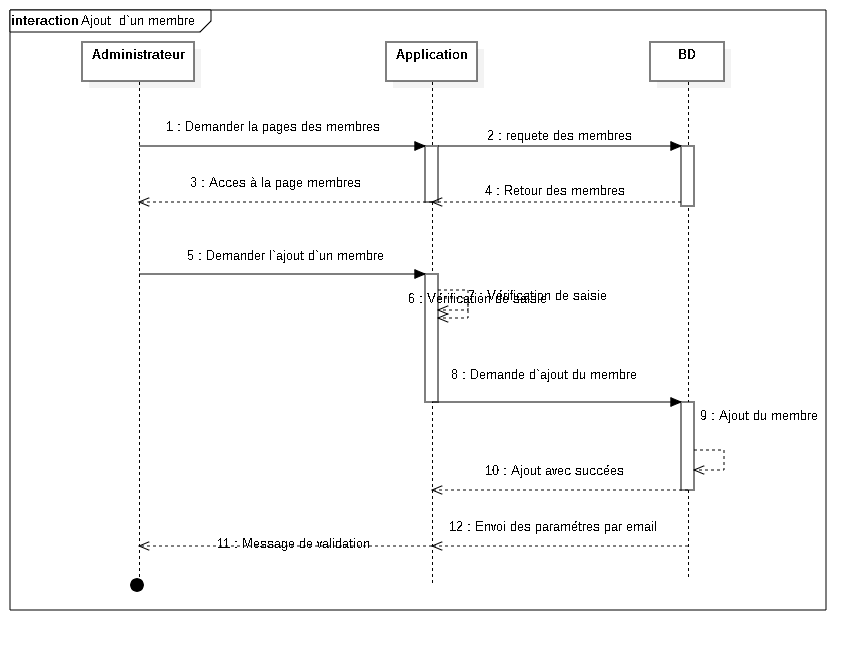
\includegraphics[width=14cm,height=10cm]{./figures/seq/E.png}
\caption{Cr\'{e}ation d'un membre.}
\end{figure}

\subsubsection{Sch\'{e}ma}
\begin{table}

\begin{tabular}{|l|l|l|l|l|l|}
\hline
Field        & Type         & Null & Key & Default            & Extra            \\
\hline
id           & int(11)      & NO   & PRI & NULL               & auto\_increment  \\
\hline
login        & varchar(30)  & YES  &     & NULL               &                  \\
\hline
password     & varchar(15)  & YES  &     & NULL               &                  \\
\hline
firstname    & varchar(50)  & YES  &     & NULL               &                  \\
\hline
lastname     & varchar(30)  & YES  &     & NULL               &                  \\
\hline
email        & varchar(100) & YES  &     & NULL               &                  \\
\hline
hiredate     & datetime     & YES  &     & CURRENT\_TIMESTAMP &                  \\
\hline
color        & varchar(6)   & YES  &     & NULL               &                  \\
\hline
projects\_id & int(11)      & YES  & MUL & NULL               &                  \\
\hline
pname        & varchar(50)  & YES  &     & NULL               &                  \\
\hline
\end{tabular}
\centering
\caption{Tasks}
\end{table}

\subsubsection{Test} 

Si un simple membre est authentifi\'{e} par son mot de passe il sera amen\'{e}e \`{a}
l'interface \guillemotleft{} gestion de taches \guillemotright{} dans laquelle il peut modifier l'\'{e}tat des
taches .(ToDo ,Doing,Done ) et La progression des taches .

\FloatBarrier
\begin{figure}[H]
\center
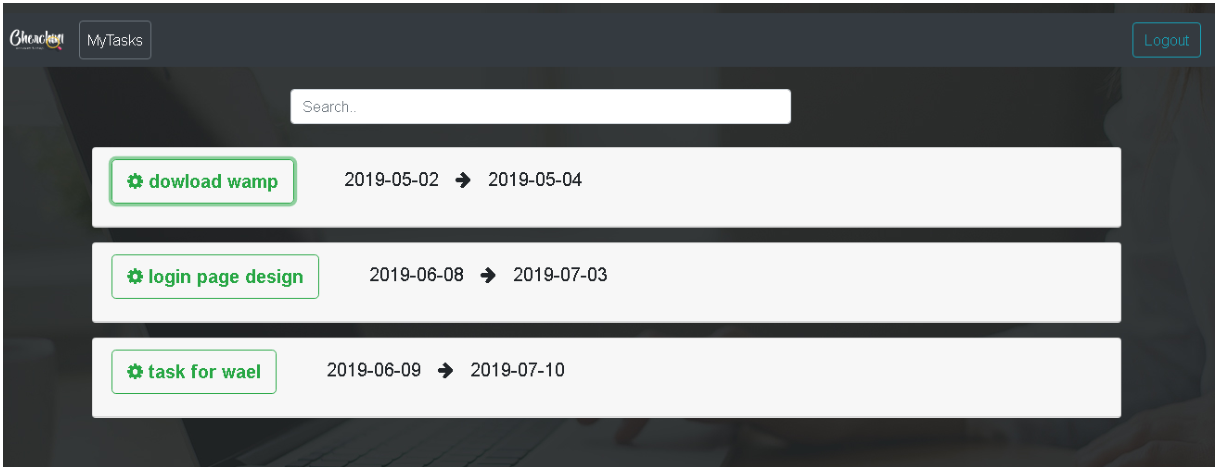
\includegraphics[width=11cm,height=7cm]{./figures/pres/2.png}
\caption{Espace membre.1.}

\end{figure}
\FloatBarrier

\FloatBarrier
\begin{figure}[H]
\center
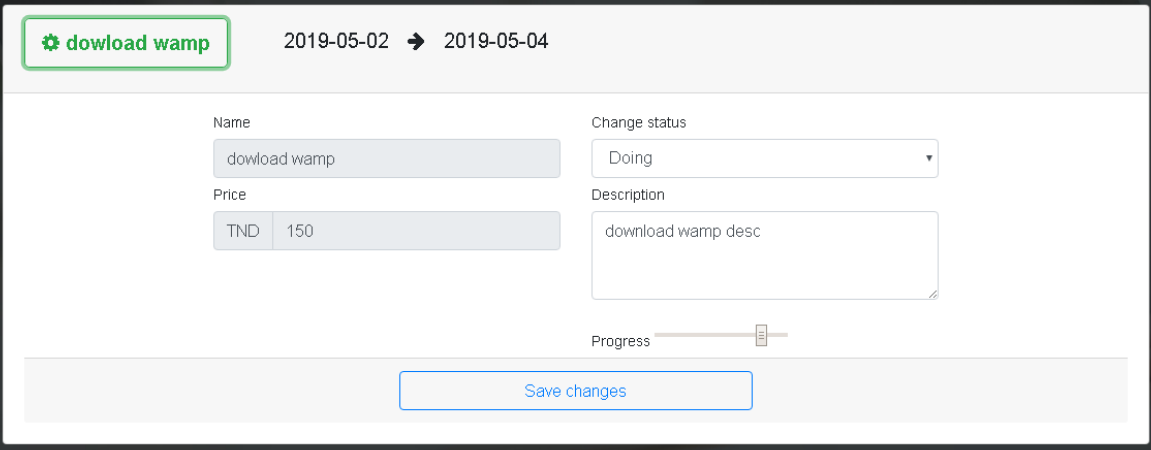
\includegraphics[width=11cm,height=7cm]{./figures/pres/3.png}
\caption{Espace membre.2.}

\end{figure}
\FloatBarrier